\chapter{Data}
\label{c:data}
\index{data|hyperbf}

A \tao \vn{``datum''} is a parameter associated with a lattice that is used in lattice correction or
design (\sref{c:opti}). Example data includes the vertical orbit at a particular position or the
horizontal emittance of a storage ring. This chapter explains how data is organized in \tao while
Section~\sref{s:init.data} explains how, in an initialization file, to define the structures that
hold the data.  When running \tao, the \vn{show data} (\sref{s:show}) command can be used to view
information about the data.


%------------------------------------------------------------------------
\section{Data Organization}
\label{s:data.org}

\begin{figure}
  \centering
  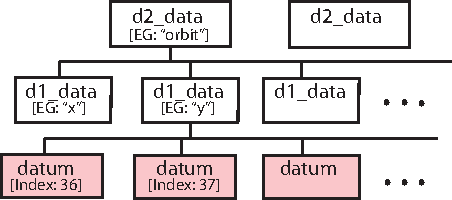
\includegraphics[width=4in]{data-tree.pdf}
  \caption[Data tree structure]
{A \vn{d2_data} structure holds a set of \vn{d1_data} structures. 
A \vn{d1_data} structure holds an array of datums.}
  \label{f:data.tree}
\end{figure}

\index{d2_data}\index{d1_data}
The horizontal orbit at a particular BPM is an example of an
individual \vn{datum}.  For ease of manipulation, arrays of datums are
grouped into what is called a \vn{d1_data} structure. Furthermore,
sets of \vn{d1_data} structures are grouped into what is called a
\vn{d2_data} structure.  This is illustrated in
Figure~\ref{f:data.tree}.  For example, a \vn{d2_data} structure for
orbit data could contain two \vn{d1_data} structures --- one
\vn{d1_data} structure for the horizontal orbit data and another
\vn{d1_data} structure for the vertical orbit data. Each datum of,
say, the horizontal orbit \vn{d1_data} structure would then correspond
to the horizontal orbit at some point in the machine.

When issuing \tao commands, all the
data associated with a \vn{d2_data} structure is specified using the
\vn{d2_data} structure's \vn{name}.  The data associated with a
\vn{d1_data} structure is specified using the format
\begin{example}
  d2_name.d1_name
\end{example}
For example, if a \vn{d2_data} structure has the
name ``\vn{orbit}'', and one of its \vn{d1_data} structures has the
name ``\vn{x}'', then \tao commands that refer to the data in this
\vn{d1_data} structure use the name ``\vn{orbit.x}''. Sometimes there
is only one \vn{d1_data} structure for a given \vn{d2_data}
structure. In this case the data can be referred to simply by using
the \vn{d2_data} structure's name. The individual datums can be
referred to using the notation
\begin{example}
  <d2_name>.<d1_name>[<list_of_datum_indexes>]
\end{example}
For example, \vn{orbit.x[10]} refers to the horizontal orbit datum
with index 10. Notice that the beginning (lowest) datum index is user
selectable and is therefore not necessarily 1. 

Period characters are not allowed in both the \vn{d2_data} and \vn{d1_data} names.

It is important to note that the name given to \vn{d2_data} and \vn{d1_data}
structures is arbitrary and does not have to correspond to the 
type of data contained in the 
structures. In fact, a \vn{d1_data} array can contain heterogeneous data types.
Thus, for example, it is perfectly permissible (but definitely not recommended) 
to set up the data structures so that, say, \vn{orbit.x[10]} 
is the $a$-mode emittance at a certain element and \vn{orbit.x[11]}
is the $b$-mode beta function at the same element.

Ranges of data can be referred to using using a comma \vn{,} to
separate the indexes combined with the notation \vn{n1:n2} to specify
all the datums between \vn{n1} and \vn{n2} inclusive. For example
\begin{example}
  orbit.x[3:6,23]
\end{example}
refers to datums 3, 4, 5, 6, and 23. 

If multiple universes are present, then, as explained in
\sref{s:universe}, the prefix \vn{"@"} may be used to specify which
universe the data applies to. The general notation is
\begin{example}
  [<universe_range>]@<d2_name>.<d1_name>[<datum_index>]
\end{example}
Examples:
\begin{example}
  [2:4,7]@orbit.x ! The \vn{orbit.x} data in universes 2, 3, 4 and 7.
  [2]@orbit.x     ! The \vn{orbit.x} data in universe 2. 
  2@orbit.x       ! Same as "2@orbit.x".
  orbit.x         ! The \vn{orbit.x} data in the current default universe.
  -1@orbit.x      ! Same as "orbit.x".
\end{example}

As explained in Section~\sref{s:data.anatomy}, each individual datum
has a number of components. The syntax to refer to a component is:
\begin{example}
  d2_name.d1_name[datum_index]|component
\end{example}
For example:
\begin{example}
  orbit.x[3:10]|meas     ! The measured data values
\end{example}

In referring to datums, a ``\vn{*}'' can be used as a wild card to 
denote ``all''. Thus:
\begin{example}
  *@orbit.x       ! The \vn{orbit.x} data in all universes.
  *               ! All the data in the current default universe.
  *.*             ! Same as "*"
  *@*             ! All the data in all the universes. 
  *@*.*           ! Same as "*@*"
  orbit.x[*]|meas ! All measured values of orbit.x
  orbit.x[]|meas  ! No values. That is, the empty set.
  orbit.x|meas    ! Same as orbit.x[*]|meas.
\end{example}
The last example shows that when referring to an entire block of data
encompassed by a \vn{d1_data} structure, the \vn{[*]} can be omitted.

%------------------------------------------------------------------------
\section{Anatomy of a Datum}
\label{s:data.anatomy}

Each datum has a number of components associated with it:
\begin{example}
  data_type        ! Character: Type of data: "orbit.x", etc.
  ele_name         ! Character: Name of lattice element where datum is evaluated.
  ele_start_name   ! Character: Name of starting lattice element in a range.
  ele_ref_name     ! Character: Name of reference lattice element.
  merit_type       ! Character: Type of constraint: "target", "max", etc.
  data_source      ! Character: How the datum is calculated. "lat", "beam", etc.
  ix_ele           ! Integer: Index of "ele" in the lattice element list.
  ix_branch        ! Integer: Lattice branch index.
  ix_ele_start     ! Integer: Index of "ele_start" in the lattice element list.
  ix_ele_ref       ! Integer: Index of "ele_ref" in the lattice element list.
  ix_ele_merit     ! Integer: Lattice index where merit is evaluated.
  ix_d1            ! Integer: Index number in d1_data structure
  ix_data          ! Integer: Index in the global data array
  ix_dModel        ! Integer: Row number in the dModel_dVar derivative matrix.
  ix_bunch         ! Integer: Bunch number to get the data from.
  eval_point       ! Character/integer: Evaluation point relative to the lattice element.
  meas             ! Real: Measured datum value. 
  ref              ! Real: Measured datum value from the reference data set.
  model            ! Real: Datum value as calculated from the model.
  design           ! Real: What the datum value is in the design lattice.
  old              ! Real: Used by \tao to save the model at some previous time.
  base             ! Real: The value as calculated from the base model.
  fit              ! Real: This value is not used by \tao.
  invalid          ! Real: The value used for delta_merit if good_model = False.
  delta_merit      ! Real: Diff used to calculate the merit function term 
  weight           ! Real: Weight for the merit function term
  merit            ! Real: Merit function term value: weight * delta^2
  s                ! Real: longitudinal position of ele.
  s_offset         ! Real: Offset of the evaluation point.
  exists           ! Logical: Does the datum exist?
  good_model       ! Logical: Does the model  component contain a valid value?
  good_design      ! Logical: Does the design component contain a valid value?
  good_base        ! Logical: Does the base   component contain a valid value?
  good_meas        ! Logical: Does the meas   component contain a valid value?
  good_ref         ! Logical: Does the ref    component contain a valid value?
  good_user        ! Logical: Does the user want this datum used in optimization?
  good_opt         ! Logical: Can be used in Tao extensions.
  good_plot        ! Logical: Can be used in Tao extensions.
  useit_plot       ! Logical: Is this datum to be used in plotting?
  useit_opt        ! Logical: Is this datum to be used for optimization?
\end{example}
When running \tao, the \vn{show data}
(\sref{s:show}) command can be used to view the components of a datum. 
The \vn{set} command (\sref{s:set}) can be used to set some of these components.

\begin{description}
  \item[base] \Newline
The value of the datum as calculated from the base lattice (\sref{s:datum.values}).
  \item[data_source] \Newline
The \vn{data_source} component specifies where the data is coming from
(\sref{s:data.source}).
  \item[data_type] \Newline
The type of data (\sref{s:data.types}). For example, \vn{beta.a}. At startup, if the
\vn{data_type} is not specified, it is set to \vn{<d2_name>.<d1_name>} where
\vn{<d2_name>} is the name of the associated \vn{d2} data structure and \vn{<d1_name>} is 
the name of the associated \vn{d1} data structure (\sref{s:init.data}).
  \item[delta_merit] \Newline
Difference used to calculate the contribution of the datum to the merit function (\sref{s:lattice.correction}).
  \item[design] \Newline
The value of the datum as calculated from the design lattice (\sref{s:datum.values}).
  \item[ele_name] \Newline
Name of the associated lattice element where the datum is evaluated
(\sref{s:datum.opt}). Also see \vn{eval_point} and \vn{s_offset} components.
  \item[ele_start_name] \Newline
Starting element of a range of lattice elements (\sref{s:data.lat.ele}).
  \item[ele_ref_name] \Newline
Reference lattice element (\sref{s:data.lat.ele}).
  \item[eval_point] \Newline
Used with \vn{s_offset} to determine where the datum is evaluated at (\sref{s:dat.eval}).
  \item[exists] \Newline
Set by \tao to True if the datum exists (\sref{s:datum.opt}). 
  \item[fit] \Newline
Not used by \tao. Can be used with custom code.
  \item[good_base] \Newline
Set by \tao. Is the \vn{base} value valid?
  \item[good_design] \Newline
Set by \tao. Is the \vn{design} value valid?
  \item[good_meas] \Newline
Set by \tao. Is the \vn{meas} value valid?
  \item[good_model] \Newline
Set by the user. Is the \vn{meas} value valid?
  \item[good_opt] \Newline
Set by the user. Is the datum valid for optimization?
  \item[good_plot] \Newline
Set by the user. Is the datum to be used in plotting?
  \item[good_ref] \Newline
Set by the user. Is the \vn{ref} value valid?
  \item[good_user] \Newline
Set by the user. Is the datum valid for optimization or plotting?
  \item[invalid] \Newline
The value used for \vn{delta_merit} if good_model = False. 
  \item[ix_branch] \Newline
The index of the lattice branch that contains \vn{ele}, \vn{ref_ele}, and \vn{start_ele}.
  \item[ix_ele] \Newline
Index of the lattice element where the datum is evaluated at. 
  \item[ix_ele_start] \Newline
Index of the start element.
  \item[ix_ele_ref] \Newline
Index of the reference element.
  \item[ix_ele_merit] \Newline
Set by \tao. When the \vn{merit_type} is set to \vn{max} or \vn{min} and there is a range
of elements that over which the there is an evaluation, ix_ele_merit is set to the element
where the value is the \vn{max} or \vn{min}.
  \item[ix_d1] \Newline
Index of the associated \vn{d1_data} array.
  \item[ix_data] \Newline
For convenience, all the datums of a given universe are put into one large array. \vn{ix_data} is the index
of the datum in this array. This is useful for debugging purposes.
  \item[ix_dModel] \Newline
For optimization, \tao creates a derivative matrix dMerit_i/dVar_j. \vn{ix_dmodel} is set
to the i\Th column of this matrix. This is useful for debugging purposes
  \item[ix_bunch] \Newline
For datums that have \vn{data_source} set to \vn{beam}, \vn{ix_bunch} selects which bunch
of the beam the datum is evaluated at.
  \item[meas] \Newline
The value of the datum as obtained from some measurement (\sref{s:datum.values}).
  \item[merit] \Newline
The contribution to the merit function due to this datum (\sref{s:lattice.correction}).
  \item[merit_type] \Newline
The type of merit (\sref{s:generalized.design}). 
  \item[model] \Newline
The value of the datum as calculated from the \vn{model} lattice (\sref{s:datum.values}).
  \item[old] \Newline
A datum value that was saved at some point in \tao's calculations. This value
can be ignored (\sref{s:datum.values}).
  \item[ref] \Newline
The reference datum value as obtained from some reference measurement (\sref{s:datum.values}).
  \item[s] \Newline
Longitudinal $s$-position of the lattice element.
  \item[s_offset] \Newline
Offset of the evaluation point when there is an associated lattice element (\sref{s:dat.eval}).
  \item[useit_opt] \Newline
Datum is possibly valid for optimization. \vn{useit_opt} is set by \tao using the other
\vn{logicals} components. A datum is used in the optimization if both \vn{useit_opt} and
\vn{good_meas} are true.
  \item[useit_plot] \Newline
Datum is valid for plotting
  \item[weight] \Newline
Weight used in evaluating the contribution of the datum to the merit function (\sref{s:lattice.correction}).
\end{description}

%------------------------------------------------------------------------
\section{Datum values}
\label{s:datum.values}

\index{data!measured}\index{data!reference}\index{data!model}
\index{data!base}\index{data!design}
A given datum has six values associated it:
\vspace{-2ex}
\begin{description}
  \vspace{-1ex}
  \item[meas] \Newline 
The value of the datum as obtained from some measurement. This is the
target or limit value that is used when running the optimizer. When
doing lattice design, the measured value corresponds to a constraint
value (\ref{c:opti}).
  \vspace{-1ex}
  \item[base] \Newline
The datum value as calculated from the \vn{base} lattice (\sref{s:lattice}).
  \vspace{-0.5ex}
  \item[design] \Newline
The value of the datum as calculated from the \vn{design} lattice (\sref{s:lattice}).
  \vspace{-0.5ex}
  \item[fit] \Newline
The \vn{fit} value is not used by \tao directly and is available for use by custom code.
  \vspace{-0.5ex}
  \item[model] \Newline
The value of the datum as calculated from the \vn{model} lattice (\sref{s:lattice}).
  \vspace{-0.5ex}
  \item[old] \Newline
A datum value that was saved at some point in \tao's calculations. This value
can be ignored.
  \vspace{-0.5ex}
  \item[ref] \Newline
The reference datum value as obtained from some reference measurement. For example,
a measurement before some variable is varied could be designated as
the \vn{reference}, and the datum taken after the variation could be 
designated the \vn{measured} datum.
\end{description}

%------------------------------------------------------------------------
\section{Evaluation Point of a Datum}.
\label{s:dat.eval}

When the datum is to be evaluated at a specific point in the lattice, that is, when there
is an associated lattice element, the default position for evaluating the datum is at the
downstream end of the element. This evaluation point can be shifted using the
\vn{eval_point} and/or \vn{s_offset} components. 

The \vn{eval_point} component can be set to one of:
\begin{example}
  beginning   ! entrance end of lattice element.
  center      ! Center of lattice element
  end         ! Exit end of lattice element. Default.
\end{example}
The evaluation point is shifted by \vn{s_offset} from the \vn{eval_point}.

If there is a reference point, the setting of \vn{eval_point} is used to determine where
the reference point is but the setting of \vn{s_offset} is ignored.

Due to internal logic considerations, Not all \vn{data_type}s are compatible with a finite
\vn{s_offset} or a setting of \vn{eval_point} to \vn{center}. The table of \vn{data_type}s
(\sref{t:data.types}) shows which \vn{data_type}s are compatible and which are not.

Another restriction is that specifying a range of elements for evaluation (that is,
specifying \vn{ele_start_name} \sref{s:init.data}) is not compatible with a finite
\vn{s_offset} or a setting of \vn{eval_point} to \vn{center}.

%------------------------------------------------------------------------
\section{Datums in Optimization}
\label{s:datum.opt}

When using optimization for lattice correction or lattice design
(\sref{c:opti}), Individual datums can be excluded from the process
using the \vn{veto} (\sref{s:veto}), \vn{restore} (\sref{s:restore}),
and \vn{use} (\sref{s:use}) commands. These set the \vn{good_user}
component of a datum. This, combined with the setting \vn{exists},
\vn{good_meas}, \vn{good_ref}, and \vn{good_opt}
determine the setting of \vn{useit_opt} which is the component that
determines if the datum is used in the computation of the merit
function. The settings of everything but \vn{good_user} is determined
by \tao

The \vn{exists} component is set by \tao to True if the datum exists
and False otherwise. A datum may not exist if the type of datum
requires the designation of an associated element but the
\vn{ele_name} component is blank. For example, a \vn{d1_data} array
set up to hold orbit data may use a numbering scheme that fits the
lattice so that , say, datum number 34 in the array does not
correspond to an existing BPM.

The \vn{good_model} component is set according to whether a datum
value can be computed from the \vn{model} lattice. For example, If a
circular lattice is unstable, the beta function and the closed orbit
cannot be computed. Similarly, the \vn{good_design} and \vn{good_base}
components mark whether the \vn{design} and \vn{base} values
respectively are valid.

When doing optimization, the \vn{delta_merit} component is set to the
\vn{delta} value used in computing the contribution to the merit
function (\sref{s:generalized.design}). If the datum's value cannot be
computed, that is, \vn{good_model} is False, or, if the design or base
values are being used in the merit calculation, \vn{good_base} or
\vn{good_design} is False, then the \vn{invalid} component is used for
\vn{delta_merit}.

\vn{good_meas} is set True if the \vn{meas} component value is set in
the data initialization file (\sref{s:init.data}) or is set using the
\vn{set} command (\sref{s:set}). Similarly, \vn{good_ref} is set True
if the \vn{ref} component has been set. \vn{good_ref} only affects the
setting of \vn{useit_opt} if the optimization is using reference data
as set by the global variable \vn{opt_with_ref} (\sref{s:globals}).

Finally \vn{good_opt} is meant for use in custom versions of \tao
(\sref{c:custom.tao}) and is always left True by the standard \tao code.

Example of using a \vn{show data} (\sref{s:show}) to check the logicals
in a datum:
\begin{example}
  Tao> show data 3@beta[1]

  Universe:   3
  %ele_name          = IP_L0
  %ele_ref_name      =
  %ele_start_name    =
  %data_type         = beta.a
      ... etc ...
  %exists            =  T
  %good_model        =  T
  %good_meas         =  F
  %good_ref          =  F
  %good_user         =  T
  %good_opt          =  T
  %good_plot         =  F
  %useit_plot        =  F
  %useit_opt         =  F
\end{example}
Here \vn{useit_opt} is False since \vn{good_meas} is False and
\vn{good_meas} is False since the \vn{meas} value of the datum (not
shown) was not set in the \tao initialization file.

%------------------------------------------------------------------------
\section{Data_source}
\index{data!data_source}
\label{s:data.source}

The \vn{data_source} component specifies where the data is 
coming from. Possible values are:
\begin{example}
  "beam"        ! Data from from multiparticle beam distribution
  "data"        ! Data from from a \tao datum in a data array.
  "lat"         ! Data from from the lattice.
\end{example}
If \vn{data_source} is set to \vn{"beam"}, the data is calculated
using multiparticle tracking.  If \vn{data_source} is set to
\vn{"lat"}, the data is calculated using the ``lattice'' which here
means everything {\em but} multiparticle tracking In particular, the "\vn{lat}" \vn{data_source}
includes data derived from single particle tracking. For example, the
\vn{"beam"} based calculation of the emittance uses the bunch sigma
matrix obtained through multiparticle tracking. The \vn{"lat"} based
calculation of the emittance uses radiation integrals.

Some data types may be restricted as to which \vn{data_source} is
possible. For example, a datum with \vn{data_type} set to
\vn{n_particle_loss} must use \vn{"beam"} for the \vn{data_source}. 
Table~\ref{t:data.types} lists which \vn{data_source} values are valid
for what data types.

%------------------------------------------------------------------------
\section{Datum Evaluation and Associated Lattice Elements}
\index{data!associated lattice elements}
\label{s:data.lat.ele}

Datums can be divided up into two classes. In one class are the datums
that are \vn{``local''}, like the beam orbit, which need to be evaluated at
either a particular point are evaluated over some finite region of the
machine. Other datums, like the emittance, are \vn{``global''} and do not
have associated evaluation points.

As mentioned, \vn{local} datums may be evaluated at a specific point
or over some evaluation region, an evaluation region is used when, for
example, the maximum or minimum value over a region is wanted. To
specify an evaluation point, an \vn{evaluation element} must be
associated with a datum. The evaluation point will be at the exit end
of this element. To specify an evaluation region, a \vn{start element}
must also be associated with a datum along with the \vn{evaluation
element}. The evaluation region is from the exit end of the \vn{start
element} to the exit end of the \vn{evaluation element}.

In addition to the \vn{evaluation element} and the \vn{start element},
a \vn{local} datum may have an associated \vn{reference element}.  A
\vn{reference element} is used as a fiducial point and the datum value
is calculated relative to that point. For example, a datum value may
be the position of the \vn{evaluation element} relative to the
position of the \vn{reference element}. The evaluation point of a
\vn{reference element} is the exit end of that element.

The components in a datum corresponding to the \vn{evaluation
element}, the \vn{reference element}, and the \vn{start element}.  are
shown in Table~\ref{t:datum.elements}.  These three elements may be
specified for a datum by either setting the name component or the
index component of the datum. Using the element index over the element
name is necessary when more than one element in the lattice has the
same name.

\begin{table}[htb]
\centering
\begin{tabular}{lll}
  \toprule
  &\multicolumn{2}{c}{\it Data Component} \\ \cmidrule{2-3}
  {\it Element} & {\it name} & {\it index} \\ \midrule
  Reference Element  & \vn{ele_ref_name}   & \vn{ix_ele_ref}   \\
  Start Element      & \vn{ele_start_name} & \vn{ix_ele_start} \\
  Evaluation Element & \vn{ele_name}       & \vn{ix_ele}       \\ \bottomrule
\end{tabular}
\caption[The three lattice elements associated with a datum.]
{The three lattice elements associated with a datum may be
specified in the datum by setting the appropriate name component or by 
setting the appropriate index component.}
\label{t:datum.elements}
\end{table}

If a datum has an associated \vn{evaluation} element, but no
associated \vn{start} or \vn{reference} elements, the \vn{model} value
of that datum is the value of the \vn{data_type} at the \vn{evaluation}
element. For example, if a datum has:
\begin{example}
  data_type      = "orbit.x"
  ele_name       = "q12"
\end{example}
here the \vn{model} value of this datum will be the horizontal orbit
at the element with name \vn{q12}.

If a datum has an associated \vn{start} element, specified by either
setting the \vn{ele_start_name} or \vn{ix_ele_start} datum components, the
datum is evaluated over a region from the exit end of the \vn{start} element
to the exit end of \vn{evaluation} element. For example, if a datum has:
\begin{example}
  data_type      = "beta.a"
  ele_name       = "q12"
  ele_start_name = "q45"
  merit_type     = "max"
\end{example}
then the \vn{model} value of this datum will be the maximum value of
the a-mode beta function in the region from the exit end of the
element with name \vn{q12} to the exit end of the element with name
\vn{q45}. Notice that when a range of elements is used, a
\vn{merit_type} of \vn{target} does not make sense. 

Typically, in evaluating a datum over some region to find the maximum
or minimum, \tao will only evaluate the datum at the ends of the
elements with the assumption that this is good enough. If this is not
good enough, marker elements can be inserted into the lattice at
locations that matter. For example, the maximum or minimum of the beta
function typically occurs near the middle of a quadrupole so inserting
marker elements in the middle of quadrupoles will improve the accuracy
of finding the extremum beta.

If a datum has an associated \vn{reference} element, specified by either
setting the \vn{ele_ref_name} or \vn{ix_ele_ref} datum components, the
\vn{model} value of the datum is the value at the \vn{evaluation} element (or the value
over the range \vn{ele_start} to the \vn{evaluation} element if \vn{ele_start} is
specified), minus the \vn{model} value at \vn{ele_ref}. For example,
if a datum has:
\begin{example}
  data_type      = "beta.a"
  ele_name       = "q12"
  ele_start_name = "q45"
  ele_ref_name   = "q1"
  merit_type     = "max"
\end{example}
then the \vn{model} value of the datum will be the same as the
previous example minus the value of the a-mode beta function at the
exit end of element \vn{q1}. There are a number of exceptions to the
above rule and datum types treat the \vn{reference} element in a different
manner. For example, the \vn{r.} data type uses the \vn{reference} element
as the starting point in constructing a transfer matrix.

%------------------------------------------------------------------------
\section{Tao Data Types}\index{data!data Types}
\label{s:data.types}

The \vn{data_type} component of datum specifies what type of data the
datum represents. For example, a datum with a \vn{data_type} of
\vn{orbit.x} represents the horizontal orbit. Table~\ref{t:data.types} lists
what data types \tao knows about.

It is important to note the difference between the \vn{d2.d1} name
that is used to refer to a datum and the actual type of data, given by
\vn{data_type}, of the datum. The \vn{d2.d1} name is arbitrary and is
specified in the \tao initialization file (\sref{s:init.data}). Often,
these names do reflect the actual type of data. However, there is no
mandated relationship between the two. For example, it is perfectly
possible to set create a data set with a \vn{d2.d1} name of
\vn{orbit.x} to hold, say, global floor position data. In fact, the
datums in a given \vn{d1} array do not all have to be of the same
type. Thus the user is free to group data as s/he sees fit.

Description of the data types:

  \begin{description}

  \item[alpha.a, .b] \Newline
Twiss function \vn{alpha}.
  \item[apparent_emit.x, .y] \Newline
The apparent emittance is the emittance that one would calculate based
upon a measurement of the beam size\cite{b:emit}. It can be useful to
compare this to the true normal mode emittance. Also See the
\vn{norm_apparent_emit}, \vn{emit.} and \vn{norm_emit.} data types.
With \vn{data_source} set to \vn{"beam"}, \vn{apparent_emit.x} is
\begin{equation}
  \text{emit}_x = \frac{\sigma_{xx} - \eta_x^2 \, \sigma_{p_zp_z}}{\beta_a}
\end{equation}
with a similar equation for \vn{apparent_emit.y}. Here $\sigma$ is the beam size matrix
\begin{equation}
  \sigma_{r_1r_2} \equiv \left< r_1 \, r_2 \right>
\end{equation}
With \vn{data_source} set to \vn{"lat"}, The apparent emittance is
calculated from the true normal mode emittance and the Twiss
parameters (Cf.~ Eqs (4) and (5) of \cite{b:emit}).

  \item[beta.a, .b, .c] \Newline
Lattice normal mode betas.

  \item[beta.x, .y, .z] \Newline
Beam projected beta functions. \vn{beta.x} is defined by
\begin{equation}
  \beta.x = \frac{<x^{2}>}{\sqrt{<x^{2}> <x'^{2}> - <x x'>^{2}}}.
\end{equation}
with similar equations for the other planes.
The average \vn{<>} is over all the particles in the beam.

Note: If the beta function is calculated from the beam distribution,
the initial beam emittance must be set to something non-zero.

  \item[bpm_cbar.22a, .12a, .11b, .12b] \Newline
The normalized Cbar coupling parameters. The computed \vn{model} values include detector
misalignments, rotations, gain errors, etc. This type of datum is useful for simulating how well
actual coupling corrections are. See the \bmad manual on ``Instrumental Measurement Attributes''
for more details.

  \item[bpm_eta.x, y] \Newline
The horizontal and vertical dispersion components. The computed \vn{model} values include detector
misalignments, rotations, gain errors, etc. This type of datum is useful for simulating how well
actual dispersion corrections are. See the \bmad manual on ``Instrumental Measurement Attributes''
for more details.

  \item[bpm_orbit.x, y] \Newline
Beam Orbit. The computed \vn{model} values include detector misalignments, rotations, gain
errors, etc. This type of datum is useful for simulating how well actual orbit corrections
are. See the \bmad manual on ``Instrumental Measurement Attributes'' for more details.

  \item[bpm_phase.a, b] \Newline
Betatron phase. The computed \vn{model} values include detector misalignments, rotations, gain
errors, etc. This type of datum is useful for simulating how well actual orbit corrections
are. See the \bmad manual on ``Instrumental Measurement Attributes'' for more details.

  \item[bpm_k.22a, .12a, .11b, .12b] \Newline
Measured beam coupling components. The computed \vn{model} values include detector misalignments, rotations, gain
errors, etc. This type of datum is useful for simulating how well actual coupling corrections
are. See the \bmad manual on ``Instrumental Measurement Attributes'' for more details.

  \item[bunch_max, bunch_min.x, .px, .y, .py, .z, .pz] \Newline
Maximum or minimum phase space coordinate in a bunch, relative to its centroid.

  \item[c_mat.11, .12, .21, .22] \Newline
Coupling matrix components. The 2x2 C matrix describe the $x$-$y$ coupling of the beam.
See the \bmad manual for more details.

  \item[cbar.11, .12, .21, .22] \Newline
Normalized coupling matrix components. The 2x2 C matrix describe the $x$-$y$ coupling of the beam.
The normalized matrix is normalized by factors of $\beta$. See the \bmad manual for more details.

  \item[chrom.a, .b] \Newline
Chromaticities. Old names: \vn{chrom.dtune.a} and \vn{chrom.dtune.b}

  \item[chrom.dbeta.a, .dbeta.b] \Newline
The normalized change of the beta function with energy
$(1/\beta_{a,b})\partial\beta_{a,b}/\partial\delta$. Unlike the standard chromaticities,\vn{chrom.a} and \vn{chrom.b},
the these chromaticities are evaluated at individual elements.

  \item[chrom.deta.a, .deta.b] \Newline
The chromatic dispersion $\partial\eta_{x,y}/\partial\delta$. Unlike the standard
chromaticities,\vn{chrom.a} and \vn{chrom.b}, the these chromaticities are evaluated at
individual elements.

  \item[chrom.detap.a, .detap.b] \Newline
The chromatic dispersion derivatives $\partial\eta'_{x,y}/\partial\delta$. Unlike the standard
chromaticities,\vn{chrom.a} and \vn{chrom.b}, the these chromaticities are evaluated at
individual elements.

  \item[chrom.dphi.a, .dphi.b] \Newline
The chromatic betatron phase $\partial\phi_{a,b}/\partial\delta$. Unlike the standard
chromaticities,\vn{chrom.a} and \vn{chrom.b}, the these chromaticities are evaluated at
individual elements.

  \item[damp.j_a, .j_b, .j_z] \Newline
Damping partition numbers.

  \item[dpx_dx, dpy_dy, etc.] \Newline
Bunch sigma matrix ratios, <x px> / <$x^2$> \& Etc.

  \item[e_tot_ref] \Newline
The reference energy of the lattice. This is the same as the \vn{E_tot} attribute of a lattice element.
For the actual particle energy, use \vn{orbit.e_tot}.

  \item[element_attrib.<attrib_name>] \Newline
The \vn{element_attrib.<attrib_name>} data type is associated with the
lattice element attribute named \vn{<attrib_name>}. See the \bmad
(\cite{b:bmad}) manual for information on attribute names. For
example, to plot the dipole bend strength \vn{g}, the following
plot template (\sref{s:init.plot}) can be used:
\begin{example}
  &tao_template_plot
    plot%name = 'bend_g'
    plot%n_graph = 1
    plot%x_axis_type = 'index'
  /

  &tao_template_graph
    graph%name = 'g'
    graph%type = 'data'
    graph_index = 1
    graph%y%label = 'g'
    graph%n_curve = 1
    curve(1)%name = 'g'
    curve(1)%data_type = 'element_attrib.g'
    curve(1)%draw_line = F
  /
\end{example}

  \item[emit.a, .b, .c] \Newline
True normal mode (eigen) emittances.  With \vn{data_source} set to \vn{"beam"}, the
emittance is calculated from the beam sigma matrix. With \vn{data_source} set to
\vn{"lat"}, the normal mode emittance is calculated using the standard radiation
integrals.

  \item[emit.x, .y, .z] \Newline
``Projected'' emittances\cite{b:emit}. 
For a linear lattice, the emittance varies along the length
of the line while for a circular lattice there is a single emittance
number. 

With \vn{data_source} set to \vn{"beam"}, the emittance is calculated from the beam sigma
matrix. The formula for $\epsilon_x$ is
\begin{equation}
  \epsilon_x = \sqrt{ \wt\sigma_{xx} \, \wt\sigma_{p_xp_x} - \wt\sigma_{xp_x}^2}
\end{equation}
With a similar equation for $\epsilon_y$. Here $\wt\sigma$ is the energy normalized
beam size:
\begin{equation}
  \wt\sigma_{xx} = \langle x \, x \rangle - 
  \frac{\langle x \, p_z \rangle \, \langle x \, p_z \rangle}{\langle p_z \, p_z \rangle}
\end{equation}
with similar definitions for the other $\wt\sigma$ components. 
Note that the projected emittance is sometimes defined using
$x'$ and $y'$ in place of $p_x$ and $p_y$. However, in the vast
majority of cases, this does not appreciably affect the numeric
results.

See also the \vn{norm_emit.}, \vn{apparent_emit.}, and
\vn{norm_apparent_emit.} data types.

  \item[expression: <arithmetic_expression>] \Newline
\vn{<arithmetic_expression>} is an arithmetic expression (\sref{s:arithmetic.exp}) which
is evaluated to get the value of the datum. For example:
\begin{example}
  datum(i)%data_type = "expression: 1@ele::q10w[beta_a] - 2@ele::q10w[beta_a]"
\end{example}
With this, the value of the datum will be the difference between the a-mode beta at
element \vn{q10w} for universe 1 and universe 2. In this example, the source of both terms
in the expression is explicitly given as \vn{ele}.  This is not necessary if the
\vn{datum%data_source} is set to \vn{ele}
\begin{example}
  datum(i)%data_type = "expression: 1@q10w[beta_a] - 2@q10w[beta_a]"
  datum(i)%data_source = "ele"
\end{example}
An expression can also be used as the \vn{default_data_type}. In this case, the evaluation
point is implicit. For example:
\begin{example}
  default_data_source = "data"
  default_data_type = "expression: 1@beta.a - 2@beta.a"
\end{example}
which is equivalent to:
\begin{example}
  default_data_type = "expression: 1@data::beta.a - 2@data::beta.a"
\end{example}

To be valid, if an expression has a term with a \vn{data} source, the
expression must be evaluated after the \vn{data} source components are
evaluated. Data evaluation is done universe by universe starting with
universe 1, then universe 2, etc. Within a given universe, the order
of evaluation can be complicated but in this case a datum using an
expression will always be evaluated after any datum that appears
earlier in the initialization file.  In the last example above, the
expression terms involve an evaluation of \vn{beta.a} in universe 2.  
Therefore, this expression datum should
be in universe 2 or higher. Notice that while all datums must be
assigned a universe, in this case, since all the terms explicitly give
a universe number, the value of the datum will be independent of the
universe it is in.

In the above examples, the lattice elements involved were explicitly specified.
To apply an expression to the lattice element associated with a datum use
the syntax ``\vn{ele::\#}'' to represent the associated lattice element. Example:
\begin{example}
  default_data_type = "expression: ele::#[k1] * ele::#[l]"
  datum(1:4)%ele_name = "Q01", "Q02", "Q03", "Q04"
\end{example}
In this example the values of the four datums will the integrated quadrupole strength K1*L
of the associated lattice elements \vn{Q01} for the first datum, etc.

  \item[floor.x, .y, .z] \Newline
Position of the element in the global ``floor'' coordinate system. This is the nominal
position ignoring any misalignments. See the \bmad manual for details on the global
coordinate system. See also \vn{rel_floor.} and \vn{will.}.

  \item[floor.theta, .phi, .psi] \Newline
Orientation of the element in the global ``floor'' coordinate system. This is the nominal
position ignoring any misalignments. See the \bmad manual for details on the global
coordinate system. See also \vn{rel_floor.}.

  \item[gamma.a, .b] \Newline
Normal mode Twiss gamma function.

  \item[k.11b, .12a, .12b, .22a] \Newline
Measured beam coupling parameters. See also \vn{bpm_k.11b, ...}.

  \item[momentum] \Newline
Particle momentum amplitude.

  \item[momentum_compaction] \Newline
Momentum compaction factor. Also see \vn{r56_compaction}.

  \item[multi_turn_orbit.x, .y, .z, .px, .py, .pz] \Newline
Used for storing the orbit over many turns. Only used for plotting purposes.
See \sref{s:plot.data} for more details.

  \item[n_particle_loss] \Newline
If the reference element is not specified, \vn{n_particle_loss} gives
the number of particles lost at the evaluation element. If the
reference element is specified, \vn{n_particle_loss} gives the
cumulative loss between the exit end of the reference element and the
exit end of the evaluation element. That is, this sum does not count
any losses at the reference element itself. If neither reference nor
evaluation element is given then the total number of lost particles is
given.

  \item[norm_apparent_emit.x, .y] \Newline
Energy normalized apparent emittance. The normalization is the standard gamma factor:
\Begineq
  \text{emit}_{\text{norm}} = \gamma \, \text{emit}
\Endeq
See the \vn{apparent_emit.x, .y} data type for more details.

  \item[norm_emit.a, .b, .c] \Newline
Energy normalized normal mode emittance. The normalization is the standard gamma factor:
\Begineq
  \epsilon_{norm} = \gamma \, \epsilon
\Endeq

  \item[norm_emit.x, .y, .z] \Newline
Energy normalized projected emittance. The normalization is the standard gamma factor:
\Begineq
  \epsilon_{norm} = \gamma \, \epsilon
\Endeq

  \item[normal.<type>.$i$.<monomial>] \Newline
Components of the normal form decomposition of the one-turn-map $M$ for a ring. 
Possible settings for \vn{type} is
\begin{example}
  M, A, A_inv, dhdj, ReF, or ImF
\end{example}      
$i$ is an integer between 1 and 6, and \vn{monomial} is a six digit number that specifies
a monomial. For example: \vn{100001}. 

In the symplectic case:
\Begineq \label{normalform1}
  M = A\circ \exp\left(:h:\right)\circ A^{-1},
\Endeq
where $A$ is the nonlinear normalizing map, and $h$ is a function of the amplitudes $J_i =
(1/2)(x_i^2 + p_i^2)$ only. The amplitude dependent tune shifts are given by $\mu_i =
-dh/dJ_i$, and can be accessed through \vn{normal.dhdj}. Terms of $A$ and $A^{-1}$ can be
accessed through \vn{normal.A} and \vn{normal.A_inv}.  In the general case,
\Begineq \label{normalform2}
M = A_1\circ C \circ L \circ \exp\left(F\cdot\nabla\right)I\circ C^{-1} \circ A_1^{-1}.
\Endeq
Here $C$ is the linear map to the resonance basis: $h_\pm = x \pm i p$, $L$ is a complex
linear map, $A_1$ is the (real) first order normalizing map, and $I$ is the identity
map. All of the nonlinearities are therefore in the complex vector field $F$. The real and
imaginary parts of $L$ and $F$ can be accessed through \vn{normal.ReF}, \vn{normal.ImF},
\vn{normal.ReL}, and \vn{normal.ImL}.

  \item[null] \Newline
A \vn{null} data type is used for data where \tao is not able to calculate a model value. Such data
cannot be used in an optimization. For example, in a linac where the beam intensity is measured at
the BPMs, \tao has no model for calculating the current variation down the linac. Nevertheless, it
could be useful to read in the measured values and plot them.

  \item[orbit.amp_a, .amp_b] \Newline
``Invariant'' amplitude of the orbital motion.

  \item[orbit.norm_amp_a, .norm_amp_b] Newline
Energy normalized ``invariant'' amplitude of the orbital motion.

  \item[orbit.e_tot] \Newline
The \vn{orbit.e_tot} data type gives the total energy of a tracked particle (with
\vn{data_source} = \vn{lat}) or the average energy of a beam (with \vn{data_source} =
\vn{beam}).

Notice that this is different from the \vn{E_tot} attribute of a lattice element which
is the reference energy at that element.

  \item[orbit.x, .y, .z, .px, .py, .pz] \Newline
Orbit position and momenta

  \item[periodic.tt.$ijklm\ldots$] \Newline
This is like the \vn{tt.} datum except here the terms are from the
periodic Taylor map defined by
\Begineq
  T_p \equiv (T_0 - I_4)^{-1}
\Endeq
Here $T_p$ is the
periodic map, $T_0$ is the one-turn map from some point back to that
point, and $I_4$ is a linear map defined by the matrix
\Begineq
  I_4 \equiv 
    \begin{pmatrix}
      1 &   &   &   &   &   \\
        & 1 &   &   &   &   \\
        &   & 1 &   &   &   \\
        &   &   & 1 &   &   \\
        &   &   &   & 0 &   \\
        &   &   &   &   & 0
    \end{pmatrix}
\Endeq
The periodic map give information about the closed orbit, dispersion,
etc. For example, the zeroth order terms are the closed orbit, the r16
term gives the horizontal dispersion, etc.

If a reference lattice element is specified, the map $T_0$ will be
the transfer map from the reference element to the evaluation element.

Note: If the reference element is not specified, or if the reference
element is the same as the evaluation element, this data type cannot
be used with a linear lattice.

  \item[phase.a, .b] \Newline
Betatron phase.  If a \vn{d1_data} array has a set of
\vn{phase} datums, and if the reference element is {\em not}
specified, the average phase used for optimizations ($D$ in
\Eq{m1}) and plotting for all the datums within a \vn{d1_data}
array are set to zero by adding a fixed constant to all the datums.
This is done since, without a reference point that defines a zero
phase, the overall average phase is arbitrary and so the average phase
is taken in \tao to be zero. This can be helpful in optimizations
since one does not have to worry about arbitrary offsets between the
\vn{model} and \vn{measured} values. If the reference element is
specified then there is no arbitrary constant in the evaluation.

  \item[phase_frac.a, .b] \Newline
Fractional betatron phase. Also see the discussion under \vn{phase.a, .b}.

  \item[phase_frac_diff] \Newline
Fractional betatron phase difference between the $a$ and $b$ normal modes. 
$-\pi < d\phi_{\mbox{frac}} < \pi$

  \item[photon.intensity] \Newline
Photon total intensity.

  \item[photon.intensity_x, .intensity_y] \Newline
Photon intensity components in the horizontal and vertical planes.

  \item[photon.phase_x, .phase_y] \Newline
Photon phases in the horizontal and vertical planes.

  \item[ping_a.amp_x, .phase_x, .amp_y, .phase_y, .amp_cos_y, .amp_sin_y] \Newline
Phase and amplitude response at a BPM from turn-by-turn data acquired after the beam is
pinged. Ignoring damping, the beam response will be the sum of three components, one for
each beam oscillation eigenmode. \vn{ping_a} data is for the response at the \vn{a}-mode
frequency. 

At each BPM, the response will have a component in the \vn{x} (horizontal) and \vn{y} (vertical)
planes. If there is no coupling, vertical response for the \vn{a}-mode component is zero. The
horizontal $x_a(s, n)$ and vertical $y_a(s, n)$ \vn{a}-mode response at position $s$ and turn $n$
is
\begin{align}
  x_a(s, n) &= A_{ax}(s) \, \cos(n \, \omega_a + \phi_{ax}(s) + \phi_{a0}) \CRNO
  y_a(s, n) &= A_{ay}(s) \, \cos(n \, \omega_a + \phi_{ay}(s) + \phi_{a0})
\end{align}
where $\omega_a$ is the $a$-mode tune, $A_{ax}$ and $A_{ay}$ are the response amplitudes, $\phi_{ax}$
and $\phi_{ay}$ are the horizontal and vertical phases, and $\phi_{a0}$ is an overall phase
dependent upon how turn $n = 0$ is defined. In terms of \tao's data parameters, the correspondence
is
\begin{example}
    ping_a.amp_x     \(\longrightarrow A_{ax}\)
    ping_a.phase_x   \(\longrightarrow \phi_{ax}\)
    ping_a.amp_y     \(\longrightarrow A_{ay}\)
    ping_a.phase_y   \(\longrightarrow \phi_{ay}\)
    ping_a.amp_sin_y \(\longrightarrow A_{ay}\cdot\sin(\phi_{ay}-\phi_{ax})\)
    ping_a.amp_cos_y \(\longrightarrow A_{ay}\cdot\cos(\phi_{ay}-\phi_{ax})\)
\end{example}
In terms of how \tao analyses ping data, only differences in phases are important so $\phi_{a0}$ is
ignorable. 

The response can be related to the lattice Twiss parameters as given by Eq.~(54) of reference
\cite{b:linear.coupled}
\begin{align}
  x_a(s, n) &=  A_a(s) \, \sqrt{\beta_a(s)} \, \cos(\theta_{ax}(s,n)) , \CRNO
  y_a(s, n) &= -A_a(s) \, \sqrt{\beta_b(s)} \Bigl( \cbar{22} \, \cos(\theta_{ax}(s,n)) +
     \cbar{12} \, \sin(\theta_{ax}(s,n)) \Bigr)
  \label{xabno}
\end{align}
where
\Begineq
  \theta_{ax}(s,n) = n \, \omega_a + \phi_{ax}(s) + \phi_{a0}
\Endeq

Roughly, if the coupling is not large, the ``in-plane'' \vn{x} oscillation is insensitive to any
coupling so that \vn{ping_a.amp_x} and \vn{ping_a.phase_x} can be directly related to the Twiss
parameters computed without coupling. On the other hand, the ``out-of-plane'' \vn{y} oscillation is
a direct measure of the coupling. This can be used to measure and correct skew-quadrupole
errors. Since the design coupling in many machines is zero or very small, in such cases the
\vn{ping_a.amp_sin_y} and \vn{ping_a.amp_cos_y} datums are better for analysis as opposed to the
\vn{ping_a.amp_y} and \vn{ping_a.phase_y} datums since the value of \vn{ping_a.phase_y} is
meaningless when the local coupling, and hence \vn{ping_a.amp_y}, is zero.

For the \vn{design} and \vn{model} values of a datum, \Eq{xabno} is used with $A_a$ taken
to be unity. To be able to compare the \vn{design} and/or \vn{model} values with the
actual data stored in \vn{meas} and/or \vn{ref}, the \vn{meas} values will be multiplied by a
constant $C_m$ computed so that the average \vn{meas} value is equal to the average
\vn{model} value:
\Begineq
  C_m \, \sum \text{ping_a.amp_x}_\text{meas} = \sum \text{ping_a.amp_x}_\text{model}
\Endeq
where the sums are over all \vn{ping_a.amp_x} data points where the \vn{exists},
\vn{good_model}, \vn{good_user}, and \vn{good_meas} components (\sref{s:data.anatomy}) are
all true. The \vn{ping_a.amp_y} data points are not used for the computation of $C_m$
since, with a decoupled lattice, the \vn{model} values are zero.

There is a similar multiplier defined for the reference data. The values of these two
multipliers are shown with the \vn{show data} command.

  \item[ping_b.amp_y, .phase_y, .amp_x, .phase_x, .amp_sin_x, .amp_cos_x] \Newline
Similar to \vn{ping_a} except this is for the \vn{b}-mode component of the response.  Here
the \vn{design} and \vn{model} values are calculated from Eq.~(8) of reference
\cite{b:beta.meas}:
\begin{align}
  x_b(n) &= A_b \, \sqrt{\beta_a} \Bigl( \cbar{11} \, \cos(n \omega_b) -
     \cbar{12} \, \sin(n \omega_b) \Bigr) , \CRNO
  y_b(n) &= A_b \, \sqrt{\beta_b} \, \cos(n \omega_b) .
  \label{yabno}
\end{align}
with \vn{A_b} taken to be unity for the evaluation.

The corresponding multiplicative values are derived from \vn{ping_b.amp_y} in an analogous
fashion to the multiplicative values for the $a$-mode ping data.

  \item[r.$ij$] \Newline
Terms of the linear transfer map. $1 \le i,j \le 6$.

  \item[ \begin{tabular}{@{}l}
  rad_int.i1, .i2, .i2_e4, .i3, .i3_e7, .i4a, .i4b, .i4z, .i5a, .i5b, .i5a_e6, .i5b_e6 \\
  rad_int1.i1, .i2, .i2_e4, .i3, .i3_e7, .i4a, .i4b, .i4z, .i5a, .i5b, .i5a_e6, .i5b_e6
  \end{tabular}] \Newline
Synchrotron radiation integrals. See the \bmad manual for details.
The \vn{rad_int1.xxx} datums are the radiation integrals over a single element.
With the \vn{rad_int.xxx} datums, the integral is from \vn{ele_ref} to \vn{ele}.
\begin{example}
  .i1         ! I1 radiation integral
  .i2         ! I2 radiation integral
  .i2_e4      ! Energy normalized I2 radiation integral
  .i3         ! I3 radiation integral
  .i3_e7      ! I3 radiation integral
  .i4a        ! $a$ mode I4 radiation integral
  .i4b        ! $b$ mode I4 radiation integral
  .i4z        ! Sum of I4a, and I4b radiation integrals
  .i5a        ! $a$ mode I5 radiation integral
  .i5b        ! $b$ mode I5 radiation integral
  .i5a_e6     ! Energy normalized I5a
  .i5b_e6     ! Energy normalized I5b
\end{example}

  \item[r56_compaction] \Newline
This datum is defined to be
\Begineq
  M_{5,6} + \sum_{i=1}^4 M_{5,i} \, \eta_i
\Endeq
where $\Bf M$ is the transfer matrix between the reference element and the element where the datum
is evaluated and $\eta$ is the dispersion vector evaluated at the reference element.

This datum is closely related to the momentum compaction. When \vn{r56_compaction} is evaluated
from the start of the lattice to the end, the value of \vn{r56_compaction} will be related to the
momentum compaction via:
\begin{example}
  r56_compaction = -momentum_compaction * L
\end{example}
where \vn{L} is the length of the lattice. 

  \item[ref_time] \Newline
This is the time the reference particle passes the exit end of the element.
If the particle is ultra-relativistic then this is just $c * s$ where $s$
is the longitudinal distance from the start of the lattice.

  \item[rel_floor.x, .y, .z, .theta] \Newline
This is the global floor position at the exit end of the evaluation
element relative to the exit end of the reference element in a global
coordinate system where the exit end of the reference element is taken to be at
\vn{x = y = z = theta = phi = 0}. See the \bmad manual for details on
the global coordinate system. See also \vn{floor.} and \vn{wall.}.

  \item[sigma.x, .y, .z, .px, .py, .pz, .$ij$, .Lxy] \Newline
Beam sizes \vn{sigma.x}, \vn{sigma.px}, etc., and angular momentum
\vn{sigma.Lxy} = $<xp_x - yp_x>$ are calculated from the beam sigma matrix
if the \vn{data_source} is set to \vn{beam} and calculated from the linear
Twiss parameters if the \vn{data_source} is set to \vn{lat}.

\vn{sigma.$ij$} with $1 \le i,j,k,\ldots \le 6$ are components of the beam sigma matrix.

Irregardless of the setting of \vn{data_source}, the beam emittance and longitudinal sigma
values will be taken from the \vn{beam_init} structure (\sref{s:beam.init}) and {\em not}
any emittances or longitudinal sigma values specified in the lattice file.

  \item[t.$ijk$,  tt.$ijklm\ldots$] \Newline
Taylor map components between two points with $1 \le i,j,k,\ldots \le 6$.  The difference
between \vn{t.$ijk$} and \vn{tt.$ijklm\ldots$} is that \vn{t.$ijk$} is restricted to
exactly three indices and \vn{tt.$ijklm\ldots$} is not. \vn{t.$ijk$} is superfluous but is
keep for backwards compatibility.

Calculation of \vn{t.$ijk$} and \vn{tt.$ijklm\ldots$} datums involve symplectic
integration through lattice elements. One point to be kept in mind is that results will be
dependent upon the integration step size through an element set by the \vn{ds_step}
attribute of that element (see the \bmad manual for more details). When a smooth curve
(\sref{s:template}) is plotted for \vn{t.$ijk$} and \vn{tt.$ijklm\ldots$} data types, and
the longitudinal (\vn{"s"}) position is used for the x-axis, the integration step used in
generating the points that define this curve will be decreased if the s-distance between
points is smaller than the \vn{ds_step}.  In this case, discrepancies between the plot and
datum values may be observed.

  \item[time] \Newline
Time (in seconds) a particle or the bunch centroid is at the evaluation element.

  \item[tune.a, .b] \Newline
Tune in radians.

  \item[unstable.orbit] \Newline
The \vn{unstable.orbit} datum is used for linear lattices in an
optimization to avoid unstable solutions (\sref{s:generalized.design}).

For single particle tracking, the value of an \vn{unstable.orbit}
datum is zero if the tracked particle survives (has not been lost) up
to the evaluation element and, if it has been lost, is set to
\Begineq
 1 + i_{\mbox{ele}} - i_{\mbox{lost}} + \frac{1}{2}
 \left[ \tanh\left( \frac{r_{orbit}}{r_{lim}} - 1 \right) - E \right]
\Endeq
where $i_{\mbox{ele}}$ is the index of the evaluation element in the
lattice and $i_{\mbox{lost}}$ is the index of the element where the
particle was lost. In the above equation, $E$ is the function
\Begineq
  E = 
  \begin{cases}
    1 & \text{if the particle is lost at the exit end of the element.} \\
    0 & \text{if the particle is lost at the entrance end of the element.}
  \end{cases}
\Endeq
In the abouve equation, $r_{orbit}$ is the particle amplitude at the
point of loss and $r_{lim}$ is the aperture limit. The form of the
above equation has been choisen so that the datum value will be
monotonic with increasing stability.

The default for the evaluation element, if \vn{ele_name} nor
\vn{ix_ele} is not specified, is to use the last element in the
lattice. 

When tracking beams, the value of \vn{unstable.orbit} is the averaged
value over all particles in the bunch.

  \item[unstable.ring] \Newline
\vn{unstable.ring} is used for storage rings. The value of an
\vn{unstable.ring} datum is zero if the ring is stable and set to the
largest growth rate of all the normal modes of oscillation if the ring
is unstable. \vn{unstable.ring} is used in an optimization to avoid
unstable solutions (\sref{s:generalized.design}).

\begin{figure}
  \centering
  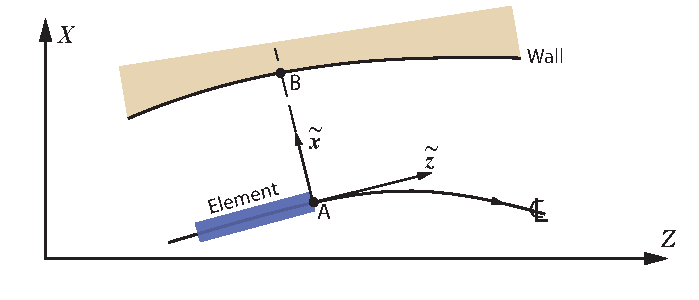
\includegraphics[width=5in]{building-wall-constraint.pdf}
  \caption[Building wall datum]
{A \vn{wall.} datum is a measure of the distance between the
centerline of a machine and the walls of the containment building.}
  \label{f:wall.constraint}
\end{figure}

  \item[velocity, velocity.x, .y, .z] \Newline
The velocity normalized by the speed of light $c$.

  \item[wall.left_side, .right_side] \Newline
The \vn{wall} data data type is used to constrain the shape of a machine to fit
inside a building's walls (\sref{s:building.wall}). The general layout is shown in
Figure~\ref{f:wall.constraint}. The machine centerline is projected onto the horizontal
$(Z, X)$ plane in the Global (floor) coordinate system. Point \vn{A} is an evaluation
point at the exit end of some element. $\wt z$ is the projection of the local $z$-axis
onto the $(Z, X)$ plane and $\wt x$ is the coordinate in the $(Z, X)$ plane perpendicular
to $\wt z$. In the typical situation, where a machine is planer (no out-of-plane bends),
the $\wt z$-axis corresponds to the local $z$-axis and the $\wt x$-axis corresponds to the
$x$-axis (see the \bmad manual for an explanation of local and global coordinate systems).

The distance from the machine at point \vn{A} to the wall is defined to be the distance
from \vn{A} to a point \vn{B} on the wall where point \vn{B} is along the $\wt x$ axis
(has $\wt z = 0$) as shown in Figure~\ref{f:wall.constraint}.

By definition, the \vn{``left side''} of the machine corresponds to be the $+\wt x$ side
and the \vn{``right side''} corresponds to be the $-\wt x$ side. That is, left and right
are relative to someone looking in the same direction as the beam is
propagating. Correspondingly, there are two wall data types: \vn{wall.left_side} and
\vn{wall.right_side}. With the \vn{wall.left_side} data type, the datum value is positive
if point \vn{B} is on the left side and negative if on the right. Vice versa for a
\vn{wall.right_side} datum.  If there are multiple wall points \vn{B}, that is, if there
are multiple points on the wall with $\wt z = 0$, the datum value will be the minimum
value. Notice that only wall sections that have a \vn{constraint} matching the datum will
be used when searching for possible points \vn{B}. If there are no wall points with $\wt z
= 0$, the datum value is set to a large number.

For \vn{wall} data there can be no reference element since this does
not make sense.

  \item[wire.<angle>] \Newline
\vn{wire} data simulates the measurement of a wire scanner. The angle
specified is the angle of the wire with respect to the horizontal
axis. The measurement then measures the second moment $<uu>$ along an
axis which is 90 degrees off of the wire axis. For example,
\vn{wire.90} is a wire scanner oriented in the vertical direction and
measures the second moment of the beam along the horizontal axis,
$<xx>$. The resultant data is not the beam size, but the beam size
squared.

  \end{description}


\index{data!calculation method}
\index{unstable.orbit}\index{beta}\index{alpha}\index{eta}\index{eta}
\index{etap}\index{phase}\index{orbit}\index{wire}\index{building wall}\index{spin}
\index{cbar}\index{coupling}\index{floor}\index{r}\index{t}\index{tt}
\index{rad_int.i5a_e6}\index{rad_int.i5b_e6}\index{s_position}\index{e_tot}
\index{unstable.ring}\index{emittance}\index{chrom}\index{norm_emittance}
\index{sigma}\index{dpx_dx}\index{dpy_dy}\index{dpz_dz}\index{dpa_da}
\index{dpb_db}\index{rad_int.i1}\index{rad_int.i2}\index{rad_int.i2_e4}
\index{rad_int.i3}\index{rad_int.i3_e7}

%----------------------------------------------------------------------------------------------

{\tt\small
\begin{longtable}{llll} 
  \caption{Predefined Data Types in Tao}
  \label{t:data.types}
  \\ \hline

  {\it Data_Type}                    & {\it Description}   & data_source & \parbox{0.5in}{\begin{tabular}{@{}l}
                                                                              Can use \\
                                                                              s_offset?
                                                                        \end{tabular}} \\ \hline\hline 
  \endfirsthead

  \caption[]{(continued)} \\ \hline
  {\it Data_Type}                    & {\it Description}   & data_source & \parbox{0.5in}{\begin{tabular}{@{}l}
                                                                              Can use \\
                                                                              s_offset?
                                                                        \end{tabular}} \\ \hline\hline 
  \endhead

  alpha.a, .b                         & Normal-Mode alpha function                & lat         & Yes \\ \hline 
  apparent_emit.x, .y                 & Apparent emittance                        & beam, lat   & No  \\ \hline

  beta.a, .b, .c                      & Normal-mode beta function                 & beam, lat   & Yes \\ \hline 
  beta.x, .y, .z                      & Projected beta function                   & beam, lat   & No  \\ \hline 
  bpm_cbar.22a, .12a, .11b, .12b      & Measured coupling                         & lat         & Yes \\ \hline
  bpm_eta.x, .y                       & Measured dispersion                       & lat         & Yes \\ \hline
  bpm_orbit.x, .y                     & Measured orbit                            & lat         & Yes \\ \hline
  bpm_phase.a, .b                     & Measured betatron phase                   & lat         & Yes \\ \hline
  bpm_k.22a, .12a, .11b, .12b         & Measured coupling                         & lat         & Yes \\ \hline
  bunch_max.x, .px, .y, .py, .z, .pz  & Max relative to centroid                  & beam        & No \\ \hline
  bunch_min.x, .px, .y, .py, .z, .pz  & Min relative to centroid                  & beam        & No \\ \hline


  c_mat.11, .12, .21, .22             & Coupling                                  & lat         & Yes \\ \hline 
  cbar.11, .12, .21, .22              & Coupling                                  & lat         & Yes \\ \hline 
  chrom.a, .b                         & Chromaticities for a ring                 & lat         & No  \\ \hline
  chrom.dbeta.a, .dbeta.b             & Normalized Chromatic beta                 & lat         & No  \\ \hline
  chrom.deta.x, .deta.y               & Chromatic dispersions                     & lat         & No  \\ \hline
  chrom.detap.x, .detap.y             & Chromatic dispersion slopes               & lat         & No  \\ \hline
  chrom.dphi.a, .dphi.b               & Chromatic betatron phase                  & lat         & No  \\ \hline

  damp.j_a, .j_b, .j_z                & Damping partition number                  & lat         & No  \\ \hline
  dpx_dx, dpx_dy, etc.                & Bunch <x px> / <$x^2$> \& Etc...          & beam        & No  \\ \hline 

  e_tot_ref                           & Lattice reference energy (eV)             & lat         & No \\ \hline
  element_attrib.<attrib_name>        & lattice element attribute                 & lat         & No  \\ \hline
  emit.a, .b, .c                      & Emittance                                 & beam, lat   & No  \\ \hline
  eta.x, .y, .z                       & Lab Frame dispersion                      & beam, lat   & Yes \\ \hline 
  eta.a, .b                           & Normal-mode dispersion                    & beam, lat   & Yes \\ \hline 
  etap.x, .y                          & Lab Frame dispersion derivative           & beam, lat   & Yes \\ \hline 
  etap.a, .b                          & $a$ \& $b$-mode dispersion derivative     & beam, lat   & Yes \\ \hline 
  expression:<expression>             & See text above                            & lat         & No  \\ \hline 

  floor.x, .y, .z                     & Global (``floor'') position               & lat         & Yes \\ \hline 
  floor.theta, .phi, .psi             & Global (``floor'') orientation            & lat         & Yes \\ \hline 

  gamma.a, .b                         & Normal-mode gamma function                & lat         & Yes \\ \hline 

  k.11b, .12a, .12b, .22a             & Coupling                                  & lat         & Yes \\ \hline 

  momentum                            & Momentum: P*C_light (eV)                  & lat         & Yes \\ \hline
  momentum_compaction                 & Momentum compaction factor                & lat         & No  \\ \hline

  \begin{tabular}{@{}l}   
    multi_turn_orbit.x, .y, .z \\ 
    multi_turn_orbit.px, .py, .pz
  \end{tabular}                       & Store orbit over many turns               & lat         & No  \\ \hline 

  n_particle_loss                     & Number of particles lost                  & beam        & No  \\ \hline 
  norm_apparent_emit.x, .y            & Normalized apparent emittance             & beam, lat   & No  \\ \hline
  norm_emit.a, .b, .c                 & Normalized beam emittance                 & beam, lat   & No  \\ \hline 
  norm_emit.x, .y, .z                 & Normalized projected emittance            & beam, lat   & No  \\ \hline 
  normal.<type>.$i$.<monomial>        & Normal Form map component                 & lat         & No  \\ \hline

  null                                & Data without model evaluation             & lat, beam   & No  \\ \hline
  
  orbit.e_tot                         & Beam energy (eV)                          & beam, lat   & Yes \\ \hline

  orbit.x, .y, .z                     & Orbit position                            & beam, lat   & Yes \\ \hline 
  orbit.px, .py, .pz                  & Orbit Momenta                             & beam, lat   & Yes \\ \hline 
  orbit.amp_a, .amp_b                 & Orbit amplitude                           & lat         & Yes \\ \hline 
  orbit.norm_amp_a, .norm_amp_b       & Energy normalized amplitude               & lat         & Yes \\ \hline 

  \begin{tabular}{@{}l}
    periodic.tt.$ijklm\ldots$ \\
    $1 \le i,j,k,\ldots \le 6$   
  \end{tabular}
                                      & Taylor term of the periodic map           & lat         & No  \\ \hline 

  phase.a, .b                         & Betatron phase                            & lat         & Yes \\ \hline 
  phase_frac.a, .b                    & \begin{tabular}{@{}l}
                                         Fractional betatron phase \\       
                                         $-\pi < \phi_{\mbox{frac}} < \pi$ \\
                                       \end{tabular}                              & lat         & No  \\ \hline 

  phase_frac_diff                     & Phase diff between $a$ and $b$ modes      & lat         & No  \\ \hline 
  photon.intensity                    & Photon total intensity                    & beam, lat   & No  \\ \hline 
  \begin{tabular}{@{}l}
    photon.intensity_x, \\
    photon.intensity_y
  \end{tabular}                       & Photon intensity components               & beam, lat   & No  \\ \hline
  photon.phase_x, .phase_y            & Photon phase                              & beam, lat   & No  \\ \hline

  \begin{tabular}{@{}l}
    ping_a.amp_x, .phase_x,      \\
    ping_a.amp_y, .phase_y       \\
  \end{tabular}                       & Amp \& phase of $a$-mode response         & lat        & No  \\ \hline

  \begin{tabular}{@{}l}
    ping_b.amp_x, .phase_x       \\
    ping_b.amp_y, .phase_y       \\
  \end{tabular}                       & Amp \& phase of $b$-mode response         & lat        & No  \\ \hline

  r.$ij$ \hspace{10pt} $1 \le i,j \le 6$
                                      & Term in linear transfer map               & lat         & No  \\ \hline 
  r56_compaction                      & R56 like compaction factor.               & lat         & No  \\ \hline
  rad_int.i1, .i2, etc.               & Lattice Radiation integrals               & lat         & No  \\ \hline
  rad_int1.i1, .i2, etc.              & Element radiation integrals               & lat         & No  \\ \hline
  ref_time                            & Reference time                            & beam, lat   & Yes \\ \hline
  rel_floor.x, .y, .z, .theta         & Relative global floor position            & lat         & No  \\ \hline 

  s_position                          & longitudinal length constraint            & lat         & Yes \\ \hline 

  \begin{tabular}{@{}l}   
    sigma.x, .y, .z \\
    sigma.px, px, .pz \\
    sigma.$ij$ \hspace{10pt} $1 \le i,j \le 6$, \\
    sigma.Lxy
  \end{tabular}                       & Bunch size                                & beam, lat   & No  \\ \hline 

  \begin{tabular}{@{}l}   
    spin.amp, .theta, .phi          \\
    spin.x, .y, .z          
  \end{tabular}                       & Particle spin                             & beam, lat   & No  \\ \hline 
  time                                & Particle time (sec)                       & beam, lat   & Yes \\ \hline
  t.$ijk$ \hspace{10pt} $1 \le i,j,k \le 6$
                                      & Term in 2\Nd order transfer map           & lat         & No  \\ \hline 
  tt.$ijklm\ldots$ \hspace{10pt} 
                                      & Term in n\Th order transfer map           & lat         & No  \\ \hline 
  tune.a, .b                          & Tune                                      & lat         & No  \\ \hline 
  unstable.orbit                      & \begin{tabular}{@{}l}   
                                          Nonzero if particles are \\
                                          lost in tracking
                                        \end{tabular}                             & lat         & No  \\ \hline
  unstable.ring                       & Nonzero if a ring is unstable             & lat         & No  \\ \hline
  velocity, velocity.x, .y, .z        & Velocity normalized by $c$                & beam, lat   & Yes \\ \hline
  wall.left_side, .right_side         & Building wall constraint                  & lat         & No  \\ \hline
  wire.<angle>                        & Wire scanner at <angle>                   & beam        & No  \\ \hline
\end{longtable}
}
